%%% In this section, you will describe all of the various artifacts that you will generate and maintain during the project life cycle. Describe the purpose of each item below, how the content will be generated, where it will be stored, how often it will be updated, etc. Replace the default text for each section with your own description. Reword this paragraph as appropriate.

\subsection{Major Documentation Deliverables}

\subsubsection{Project Charter}
%%Describe how this document will be maintained and updated (how often, under what circumstances, etc.). When will the initial version be delivered? When will the final version be delivered?
This document will be maintained and updated on a sprint-by-sprint basis after group discussion in the cases that new risks emerge, new items need to be added to the budget, etc.. The initial version of this document will be delivered on June 29, 2022, while the final version of this document will be delivered August 12, 2022.

\subsubsection{System Requirements Specification}
%Describe how this document will be maintained and updated (how often, under what circumstances, etc.). When will the initial version be delivered? When will the final version be delivered?
This document will be maintained through each update we have on our product and updated as necessary when the need for higher system requirements is needed. The initial version of this document will be delivered on July 13, 2022, while the final version of this document will be delivered August 12, 2022.

\subsubsection{Architectural Design Specification}
%Describe how this document will be maintained and updated (how often, under what circumstances, etc.). When will the initial version be delivered? When will the final version be delivered?
This document will be maintained and updated as needed when making changes to the framework of our initial design mock-up. The initial version of this document will be delivered on July 27, 2021, while the final version of this document will be delivered August 12, 2022.

\subsubsection{Detailed Design Specification}
%Describe how this document will be maintained and updated (how often, under what circumstances, etc.). When will the initial version be delivered? When will the final version be delivered?
The document will be maintained and updated any time we need to make a change to the structure of our code or to the system specifications to the hardware needed. The initial version of this document will be delivered on  , while the final version of this document will be delivered August 12, 2022.

\subsection{Recurring Sprint Items}

\subsubsection{Product Backlog}
%How will items be added to the product backlog from the SRS? How will these items be prioritized? Who makes the decision (product owner, group vote, etc.)? What software will be used to maintain and share the product backlog with team members and stakeholders?
When adding items to our product backlog we will hold a team meeting either in person or virtually through Discord to discuss whether it is added and the priority it will receive relative to the other items on the backlog currently. We will simply be using a combination of Outlook email and Discord group messaging to claim tasks and log hours for those tasks.

\subsubsection{Sprint Planning}
%How will each sprint plan be planned? How many sprints will there be (you need to look at the schedules for this course and previous Senior Design II courses during the appropriate semesters to figure this out).
Each sprint will be planned out around what immediate tasks need to get done regarding documentation and what needs to be done to progress in the development of our actual product. There will be 8 sprints total split equally between SD I and SD II.

\subsubsection{Sprint Goal}
%Who decides the sprint goal? How will you involve your customer in this process?
All members coming to consensus will be the primary decision maker on each sprint goal after group discussion and input. We will meet with the customer each sprint to ensure the sprint goal has met their requirements.

\subsubsection{Sprint Backlog}
%Who decides which product backlog items make their way into the sprint backlog? How will the backlog be maintained (collaboration software, a "scrum board", etc.)?
Each sprint we will come together as a group and decide which product backlog items will need to be added into the sprint backlog to be worked on. The sprint backlog will be maintained on through group messaging on Discord to determine what items are currently being worked on and by whom.

\subsubsection{Task Breakdown}
%How will individual tasks be assigned from the sprint backlog? Will it be up to each team member to voluntarily claim a task, or will it come from the product owner? How will time spent on tasks be documented?
Individual tasks from the sprint backlog will initially be taken on a voluntary basis and if there are still important items that must be done it will then be either done as a group or assigned to individuals.

\subsubsection{Sprint Burn Down Charts}
Which ever team member is first in generating burn down charts for each sprint. This person will be able to access the total amount of effort expended by each team member through logging hours on a shared discord server.

\begin{figure}[h!]
    \centering
    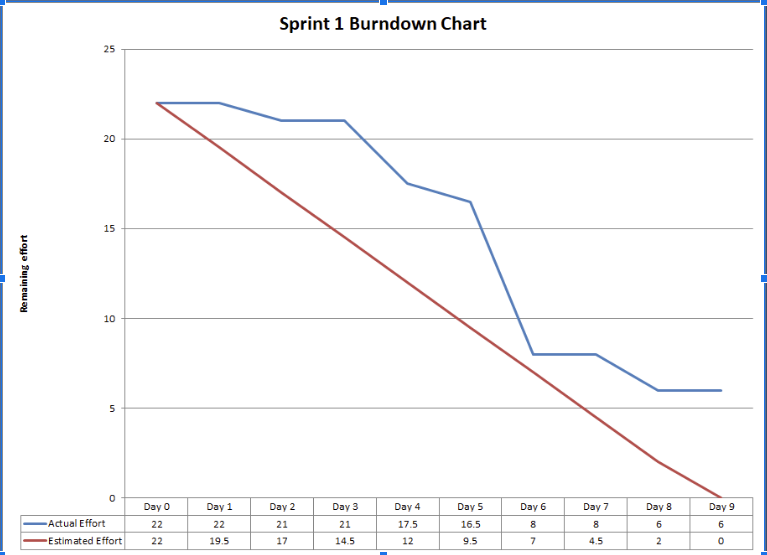
\includegraphics[width=0.5\textwidth]{images/sprint1_burndown.png}
    \caption{Example sprint burn down chart}
\end{figure}

\subsubsection{Sprint Retrospective}
%How will the sprint retrospective be handled as a team? When will this discussion happen after each sprint? What will be documented as a group and as individuals, and when will it be due?
The sprint retrospective be handled as a regular team meeting and will be held around the end of the current sprint. Meeting details will be documented within engineering notebooks per individual as normal.

\subsubsection{Individual Status Reports}
%What sort of status will be reported by each individual member, and how often will it be reported? What key items will be contained in the report?
The general status to be reported by each individual member will be the sprint backlog along with their time expenditure spent on each task that was worked on every 1.5 weeks/sprint duration. The major key items to be reported will be an individual retrospective and a peer review to conclude each sprint.

\subsubsection{Engineering Notebooks}
%How often will the engineering notebook be updated, at a minimum, by each team member? What is the minimum amount of pages that will be completed for each interval, and how long will that interval be? How will the team keep each member accountable? Who will sign of as a "witness" for each ENB page?
The engineering notebook will be updated once a week minimum, with a minimum of 1 page during the 1.5-week sprint interval. We will keep each other accountable through meetings to share new findings, updates, research, etc. weekly.

\subsection{Closeout Materials}
%The following materials, in addition to major documentation deliverables, will be provided to the customer upon project closeout. Remove this paragraph from your draft, but leave the heading.

\subsubsection{System Prototype}
%What will be included in the final system prototype? How and when will this be demonstrated? Will there be a Prototype Acceptance Test (PAT) with your customer? Will anything be demonstrated off-site? If so, will there be a Field Acceptance Test (FAT)?
The Final prototype will include a working database along with a barcode system that tracks the items. This system will also have the ability to check out items and track their whereabouts based in. Testing will be done in conjunction with the Simulation Inventory Specialist to ensure that all requirements are met.

\subsubsection{Project Poster}
%What will be included on the poster, what will be the final dimensions, and when will it be delivered?
Poster will Include screenshots of the GUI as well as information related to the Nursing Simulation Classes to better inform others of what this Application will do. Poster will be on a regular 36" by 48" poster board.

\subsubsection{Web Page}
%What will be included on the project web page? Will it be accessible to the public? When will this be delivered? Will it be updated throughout the project, or just provided at closeout (at a minimum, you need to provide a simple web page at the end).
Web page will include some simple instructions for how to operate the inventory system for easy reference of users. Will be created at the end of November.

\subsubsection{Demo Video}
%What will be shown in the demo video(s)? Will you include a B-reel footage for future video cuts? Approximately how long will the video(s) be, and what topics will be covered?
The Demo video will include a screen capture of items being added to the inventory. Also shown in the Demo will be the checking out of items as well as the showing of their whereabouts. The final portion of the demo video will have an item being removed from the system or "Surplus".

\subsubsection{Source Code}
%How will your source code be maintained? What version control system will you adopt? Will source code be provided to the customer, or binaries only? If source code is provided, how will it be turned over to the customer? Will the project be open sourced to the general public? If so, what are the license terms (GNU, GPL, MIT, etc.). Where will the license terms be listed (in each source file, in a single readme file, etc.).

Our project will utilize GitHub to store code and also as our versioning control system. The code will be open sourced under the MIT licensing terms in the parent folder of the git repository. Our customer will not be receiving the source code and will just receive the built application as the product.


\subsubsection{Source Code Documentation}
%What documentation standards will be employed? Will you use tools to generate the documentation (Doxygen, Javadocs, etc.). In what format will the final documentation be provided (PDF, browsable HTML, etc.)?
For documentation on this project, the scrum standard will be followed. Documentation such as user guides, installation notes, and release notes will be provided along with the final documentation in a PDF format.

\subsubsection{Hardware Schematics}
%Will you be creating printed circuit boards (PCBs) or wiring components together? If so, list each applicable schematic and what sort of data it will contain (PCB layout, wiring diagram, etc.). If your project is purely software, omit this section.
Our project is purely software so this section does not apply.

\subsubsection{CAD files}
%Will the project involve any mechanical design, such as 3D printed or laser-cut parts? If so, what software will you use to generate the files and what file formats will you provide in your closeout materials (STL, STEP, OBJ, etc.). If your project is purely software, omit this section.
Our project is purely software so this section does not apply.

\subsubsection{Installation Scripts}
%How will the customer deploy software to new installations? Will you provide installation scripts, install programs, or any other tools to improve the process? Will there be multiple scripts provided (perhaps separate scripts for the graphical front end and back end server software)?

The customer will be provided with an installation launcher that will allow the customer to simply install the application without the overhead of understanding CLI commands.

\subsubsection{User Manual}
%Will you customer need a printed or digital user manual? Will they need a setup video? Decide now what will be provided and discuss.
The Customer will be provided a digital user manual as well as a setup video going over the different actions that are capable within the application.
